\subsubsection{Reconnaissance de formes dessinées}

Un des objectifs de notre projet était de détecter des formes simples dans une vidéo. Ci-dessous sont présentés deux exemples de formes simples.\\

\begin{center}
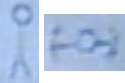
\includegraphics[scale=1]{images/templates.png}
\captionof{figure}{\\Exemples de templates}
\end{center}

Afin de reconnaître ces pictogrammes dans la vidéo, nous avons mis en place un système de détecteur.\\

Nous avons implémenté deux détecteurs différents. Le premier s'appuie sur du template matching pour reconnaître une forme. Le second utilise les descripteurs SURF.\\

Pour faire ainsi, nous avons mis en place une classe abstraite \texttt{Detector} qui présente les fonctions de base d'un détecteur, à savoir ajouter, récupérer ou supprimer un template, et définit la fonction permettant de lancer la détection.
Chacun de nos détecteurs (\texttt{MatchingDetector} et \texttt{SurfDetector}) doit donc implémenter cette fonction de détection.

\paragraph{Template matching\vspace{0.5cm}\\}

Notre premier détecteur est le \texttt{MatchingDetector}, qui utilise l'algorithme de template matching.\\

L'algorithme de template matching consiste à faire glisser un template sur la surface de l'image, et de calculer un score de "corrélation" entre le template et la zone qu'il recouvre.\\

\begin{center}
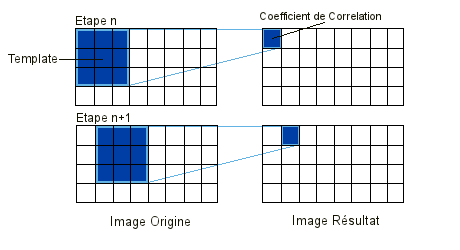
\includegraphics[width=\textwidth]{images/templateMatching.png}
\captionof{figure}{Principe du Template Matching}
\end{center}

Pour effectuer cette procédure, nous parcourons la liste des templates du détecteur. Pour chacun de ces templates, nous avons utilisé la fonction \texttt{cvMatchTemplate} d'OpenCV pour calculer une image de corrélation entre le template et l'image tirée de la vidéo, qui montre les endroits où le template a le plus correspondu à l'image. Après normalisation, nous parcourons cette image pour récupérer le minimum (ou maximum suivant la méthode passée en paramètre à \texttt{cvMatchTemplate}), ce minimum/maximum est l'endroit de meilleur matching. Nous stockons alors le quadruplet $(x,y,w,h)$ avec :
\begin{description}
\item[x,y] Les coordonnées du point de meilleur matching correspondant au coin supérieur gauche de la zone rectangulaire représentant l'objet détecté.
\item[w,h] Les dimensions du template, correspondant aux dimensions de la zone rectangulaire représentant l'objet détecté.\\
\end{description}

Une fois la position du meilleur matching récupérée, nous retirons de l'image source la zone rectangulaire décrite par le quadruplet $(x,y,w,h)$. Cette étape permet d'éviter que deux templates trop proches détectent le même objet alors que deux objets sont valides (exemple : Sur un dessin, deux bonhommes sont dessinés. Avec deux templates de bonhomme, il est possible que les deux matchings trouvent comme meilleur résultat le premier bonhomme et ne détectent pas le second. Notre étape de suppression permet de faire en sorte qu'une fois que le premier matching a détecté le premier bonhomme, celui-ci n'est plus pris en compte pour les détections des autres templates. On augmente ainsi les chances de détecter tous les objets de l'image.)\\

Une fois tous les templates parcourus, nous retournons l'ensemble des quadruplets $(x,y,w,h)$ correspondant aux détections.\\

Un des défauts de notre \texttt{MatchingDetector} est que le retour de\\ \texttt{cvMatchTemplate} ne nous permet pas de calculer un seuil de confiance pour accepter ou rejeter le résultat du matching. On peut récupérer l'endroit où le template a le plus correspondu à l'image, mais on ne sait pas si il a matché à 99\% où à 10\%.\\

Ce défaut, couplé à la normalisation du résultat de \texttt{cvMatchTemplate} (première tentative, infructueuse, de déterminer un seuil de confiance) entraîne un faux positif lorsque le template ne matche pas un des objets de l'image.\\ Le problème est double : pour le moment, nous avons un template = un résultat. On a donc forcément des faux positifs lorsque le nombre de templates d'un type d'objet dépasse le nombre d'objets de ce type du dessin, ou quand le template ne matche pas à un des objets du dessin. Nous avons également des faux négatifs, donc des objets qui ne sont pas détectés, lorsque le nombre de templates d'un type d'objet est inférieur au nombre d'objets de ce type dans le dessin.\\

Une solution au problème serait d'arriver à calculer un indice de confiance du matching. Si cet indice de confiance ne dépasse pas un seuil à définir, on ne prend pas en compte le résultat du matching pour ce template.\\

Cette solution permet de boucler sur un template jusqu'à ce que l'indice de confiance calculé ne passe plus le seuil. Cela permet d'avoir un template par type d'objet, et non un template = un résultat positif comme à présent. Avec peu de templates de bonhomme, on pourrait détecter un grand nombre de bonshommes dans le dessin. On réduirait ainsi le problème de faux négatifs lorsque le nombre de templates d'un type d'objet est inférieur au nombre d'objets de ce type. Et comme on ne prend pas en compte les matchings qui ne passent pas le seuil, on réduit également le nombre de faux positifs.\\


\paragraph{SURF : Speeded Up Robust Features\\}

Le second type de détecteur que nous avons implémenté se base sur les descripteurs SURF.\\

L'algorithme SURF permet de déterminer des points d'intérêt dans une image, ainsi que de détecter ces points dans une autre image. L'intérêt de SURF est qu'il n'est ni sensible à la rotation ni à la mise à l'échelle.\\

Dans OpenCV, SURF est implémenté par la classe \texttt{ObjectFinder}, notre \texttt{SurfDetector} utilise donc cette classe pour détecter les objets.\\

Dans un premier temps, le détecteur est initialisé avec la liste des templates que nous voulons détecter, c'est à cette étape que les descripteurs des templates sont calculés. Ce sont ces descripteurs qui sont utilisés, et comparés à ceux trouvés dans l'image pour déterminer si un objet est présent dans l'image.\\

La fonction qui fait cette détection est \texttt{find} de la classe \texttt{ObjectFinder}. Cette fonction calcule la liste des descripteurs contenus dans l'image, et compare ensuite ces descripteurs à ceux trouvés dans les templates. Si un objet est détecté, elle retourne ensuite un ensemble de points qui correspondent aux coins du polygone englobant l'objet détecté. À partir de ces points, nous calculons le quadruplet $(x,y,w,h)$ présenté dans la partie précédente pour garder une cohérence entre les retours des différents détecteurs.\\

Le principal problème que nous avons rencontré avec ce détecteur utilisant SURF, est que la vidéo est de mauvaise qualité. Les templates que nous utilisons étant tirés de la vidéo, l'algorithme de calcul de descripteurs ne retourne que très peu de résultats, pas suffisamment pour pouvoir détecter un objet. Après test sur des images en haute qualité, nous avons pu vérifier que le détecteur repère bien des objets qui ont subi une rotation, ou qui ont changé d'échelle.\\

\begin{center}
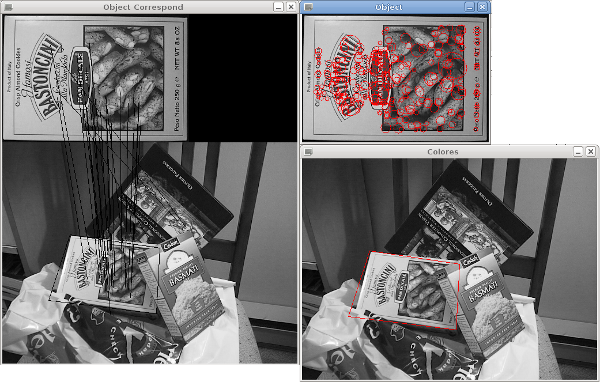
\includegraphics[width=\textwidth]{images/findobj.png}
\captionof{figure}{Exemple de SURF}
\end{center}

Sur la figure ci-dessus, nous pouvons voir différentes étapes de l'algorithme SURF. La partie gauche présente la correspondance entre les descripteurs du modèle de boite, et la scène contenant la boite parmi divers objets. La partie droite de la figure présente elle deux choses : elle présente en haut les marqueurs trouvés sur la boite, et en bas montre le résultat de la détection.\\